\documentclass[../../main.tex]{subfiles}

\begin{document}
While simulated data are very useful since a ground truth can be used to determine accuracy, it is important to see also how well SCarborSNV works on real data.
This however requires a significant amount of preprocessing to get the real data from a sequencing machine to be ready for SCarborSNV and its similar tools to use.
Furthermore, real datasets have significantly longer genomes than the simulated examples above.
Since Sci$\Phi$ in particular takes so long to run, for practical reasons we only compare SCarborSNV on a portion of the genome by truncating the input pileup file.
While this disadvantages both phylogeny aware algorithms by reducing the available kinship information, it should disadvantage them equally.
It should be noted, however, that this restriction may make Monovar perform comparatively better than if this test were to be done on the full genome.

\subsubsection*{Data and preprocessing}
We here use the same dataset used by \cite{sciphi} (accession: SRA053195), which includes DNA sequencing data from 16 single tumor cells from a triple negative breast cancer patient~\cite{DATA}.
The raw FASTQ files were downloaded from the NCBI Sequence Read Archive using the SRAToolkit's fastq-dump program.

Next we indexed the hg19 human genome with the BWA index command, and then used BWA-mem to perform the Burrows-Wheeler alignment, aligning the reads from each of the cell samples to the now indexed hg19~\cite{BWAMEM}.
We then added unique read-group identifiers to each aligned BAM file created by BWA using the Picard tool `AddOrReplaceReadGroups'.
We also used Picard to remove spurious duplicate reads, and sorted the BAM files with Samtools sort~\cite{samtools}.

Using the Genome Anlaysis Toolkit (GATK) version 3, we then locally realigned the reads around indels using the RealignerTargetCreator and IndelRealigner tools~\cite{gatk1}.
These tools have been depracated from GATK version 4 and removed from the GATK data preparation best practices as GATK now recommends variant callers that perform haplotype assembly and do not require realignment~\cite{gatk2}.
Since SCarborSNV and other SCS callers do not perform this operation we have chosen to do the local realignment.

Finally we perform base quality score recalibration using GATK version 4.
This process uses machine learning to adjust the read quality scores from the original sequencer output by detecting non-biological artifacts ifrom the sequencing machine that may have systematically affected the read quality scores~\cite{gatk1}.

\subsection*{Cancer cell results}
We analyzed 13 of the 16 tumor cells in SRA053195 using Monovar, Sci$\Phi$ and SCarborSNV.
For practical time considerations, we only analyzed the first 33.6 million ($2^{25}$) sites of each cell.
Since there is no a priori way to know what mutations were actually present in this patient, we can only compare the results of the three tools.

In terms of mutations found, Figure~\ref{fig:venn} shows unique and common mutations identified by by the three different tools.
While there were some mutations that Monovar called that SCarborSNV did not, there was only 1 (???) site that Sci$\Phi$ called as variant that SCarborSNV did not.
ScarborSNV did however call many more sites as variant than the other two tools, suggesting perhaps a high rate of false positive errors and therefore low precision.
This discrepancy could hopefully be remedied by a different choice of threshold values.

\begin{figure}[h]
    \centering
    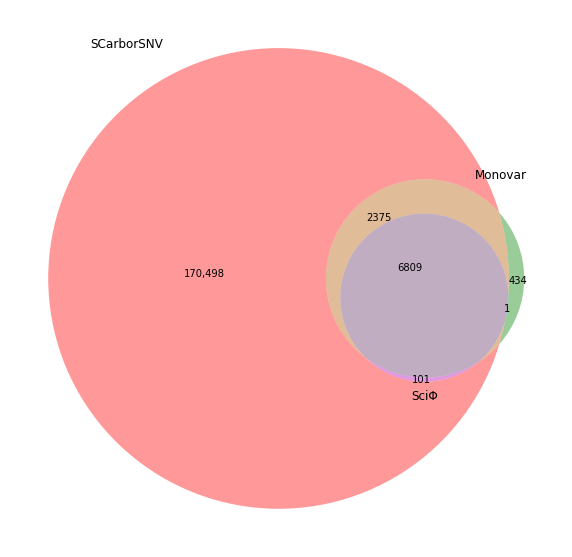
\includegraphics[width=0.9\textwidth]{sections/graphics/venndiagram}
    \caption{Venn diagram of variant sites called from the first 33.6 million sites of 13 cells in SRA053195.
    The radius of the SCarborSNV circle size has been reducedi by half to show detail in the overlapping regions.}
    \label{fig:venn}
\end{figure}


Since SCarborSNV and Sci$\Phi$ both infer phylogenies, the dendrograms of the two final inferred phylogenies are shown in Figure~\ref{fig:dendrograms}.
Both show a similar genetic structure, with about half the cells simply branching off the main trunk, with the other half together in a more heirarchical structure.

\begin{figure}[h]
    \centering
    \begin{subfigure}[b]{0.9\textwidth}
        \centering
        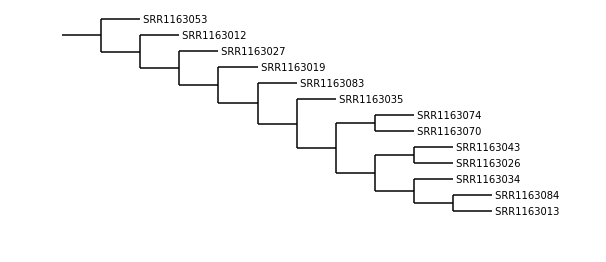
\includegraphics[width=\textwidth]{sections/graphics/SCarbor32_dendro}
        \caption{Dendrogram of tree inferred by SCarborSNV}
    \end{subfigure}
    \begin{subfigure}[b]{0.9\textwidth}
        \centering
        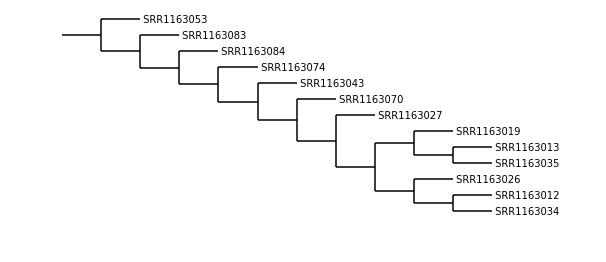
\includegraphics[width=\textwidth]{sections/graphics/SCIPHI32_dendro}
        \caption{Dendrogram of tree inferred by Sci$\Phi$}
    \end{subfigure}
    \caption{Comparison of the phylogenies inferred by SCarborSNV and Sci$\Phi$ on cells from SRA053195. For better comparison all edge lengths have been set to 1.}
    \label{fig:dendrograms}
\end{figure}

\end{document}

